\documentclass[a4paper]{article}

\usepackage{inputenc}
\usepackage[british,UKenglish]{babel}
\usepackage{amsmath}
%\usepackage{titlesec}
\usepackage{color}
\usepackage{graphicx}
\usepackage{fancyref}
\usepackage{hyperref}
\usepackage{float}
\usepackage{scrextend}
\usepackage{setspace}
\usepackage{xargs}
\usepackage{multicol}
\usepackage{nameref}

\usepackage{sectsty}
\usepackage{multicol}
\usepackage{multirow}
\usepackage[procnames]{listings}
\usepackage{appendix}

\newcommand\tab[1][1cm]{\hspace*{#1}}
\hypersetup{colorlinks=true, linkcolor=black}
\interfootnotelinepenalty=10000

\newcommand{\cleancode}[1]{\begin{addmargin}[3em]{3em}\texttt{\textcolor{cleanOrange}{#1}}\end{addmargin}}
\newcommand{\cleanstyle}[1]{\text{\textcolor{cleanOrange}{\texttt{#1}}}}


\usepackage[colorinlistoftodos,prependcaption,textsize=footnotesize]{todonotes}
\newcommandx{\commred}[2][1=]{\textcolor{Red}
{\todo[linecolor=red,backgroundcolor=red!25,bordercolor=red,#1]{#2}}}
\newcommandx{\commblue}[2][1=]{\textcolor{Blue}
{\todo[linecolor=blue,backgroundcolor=blue!25,bordercolor=blue,#1]{#2}}}
\newcommandx{\commgreen}[2][1=]{\textcolor{OliveGreen}{\todo[linecolor=OliveGreen,backgroundcolor=OliveGreen!25,bordercolor=OliveGreen,#1]{#2}}}
\newcommandx{\commpurp}[2][1=]{\textcolor{Plum}{\todo[linecolor=Plum,backgroundcolor=Plum!25,bordercolor=Plum,#1]{#2}}}

\def\code#1{{\tt #1}}

\def\note#1{\noindent{\bf [Note: #1]}}

\makeatletter
%% The "\@seccntformat" command is an auxiliary command
%% (see pp. 26f. of 'The LaTeX Companion,' 2nd. ed.)
\def\@seccntformat#1{\@ifundefined{#1@cntformat}%
   {\csname the#1\endcsname\quad}  % default
   {\csname #1@cntformat\endcsname}% enable individual control
}
\let\oldappendix\appendix %% save current definition of \appendix
\renewcommand\appendix{%
    \oldappendix
    \newcommand{\section@cntformat}{\appendixname~\thesection\quad}
}
\makeatother


% "define" Scala
\usepackage[T1]{fontenc}  
\usepackage[scaled=0.82]{beramono}  
\usepackage{microtype} 

\sbox0{\small\ttfamily A}
\edef\mybasewidth{\the\wd0 }

\lstdefinelanguage{scala}{
  morekeywords={abstract,case,catch,class,def,%
    do,else,extends,false,final,finally,%
    for,if,implicit,import,match,mixin,%
    new,null,object,override,package,%
    private,protected,requires,return,sealed,%
    super,this,throw,trait,true,try,%
    type,val,var,while,with,yield},
  sensitive=true,
  morecomment=[l]{//},
  morecomment=[n]{/*}{*/},
  morestring=[b]",
  morestring=[b]',
  morestring=[b]"""
}

\usepackage{color}
\definecolor{dkgreen}{rgb}{0,0.6,0}
\definecolor{gray}{rgb}{0.5,0.5,0.5}
\definecolor{mauve}{rgb}{0.58,0,0.82}

% Default settings for code listings
\lstset{frame=tb,
  language=scala,
  aboveskip=3mm,
  belowskip=3mm,
  showstringspaces=false,
  columns=fixed, % basewidth=\mybasewidth,
  basicstyle={\small\ttfamily},
  numbers=none,
  numberstyle=\footnotesize\color{gray},
  % identifierstyle=\color{red},
  keywordstyle=\color{blue},
  commentstyle=\color{dkgreen},
  stringstyle=\color{mauve},
  frame=single,
  breaklines=true,
  breakatwhitespace=true,
  procnamekeys={def, val, var, class, trait, object, extends},
  procnamestyle=\ttfamily\color{red},
  tabsize=2
}

\lstnewenvironment{scala}[1][]
{\lstset{language=scala,#1}}
{}
\lstnewenvironment{cpp}[1][]
{\lstset{language=C++,#1}}
{}
\lstnewenvironment{bash}[1][]
{\lstset{language=bash,#1}}
{}
\lstnewenvironment{verilog}[1][]
{\lstset{language=verilog,#1}}
{}



%代码段设置
\lstset{numbers=left,
basicstyle=\tiny,
numberstyle=\tiny,
keywordstyle=\color{blue!70},
commentstyle=\color{red!50!green!50!blue!50},
frame=single, rulesepcolor=\color{red!20!green!20!blue!20},
escapeinside=``
}

\graphicspath{ {images/} }
\usepackage{ctex}
\usepackage{graphicx}
\usepackage{color,framed}%文本框
\usepackage{listings}
\usepackage{caption}
\usepackage{amssymb}
\usepackage{enumerate}
\usepackage{xcolor}
\usepackage{bm} 
\usepackage{lastpage}%获得总页数
\usepackage{fancyhdr}
\usepackage{tabularx}  
\usepackage{geometry}
\usepackage{minted}
\usepackage{graphics}
\usepackage{subfigure}
\usepackage{float}
\usepackage{pdfpages}
\usepackage{pgfplots}
\pgfplotsset{width=10cm,compat=1.9}
\usepackage{multirow}
\usepackage{footnote}
\usepackage{booktabs}

%-----------------------伪代码------------------
\usepackage{algorithm}  
\usepackage{algorithmicx}  
\usepackage{algpseudocode}  
\floatname{algorithm}{Algorithm}  
\renewcommand{\algorithmicrequire}{\textbf{Input:}}  
\renewcommand{\algorithmicensure}{\textbf{Output:}} 
\usepackage{lipsum}  
\makeatletter
\newenvironment{breakablealgorithm}
  {% \begin{breakablealgorithm}
  \begin{center}
     \refstepcounter{algorithm}% New algorithm
     \hrule height.8pt depth0pt \kern2pt% \@fs@pre for \@fs@ruled
     \renewcommand{\caption}[2][\relax]{% Make a new \caption
      {\raggedright\textbf{\ALG@name~\thealgorithm} ##2\par}%
      \ifx\relax##1\relax % #1 is \relax
         \addcontentsline{loa}{algorithm}{\protect\numberline{\thealgorithm}##2}%
      \else % #1 is not \relax
         \addcontentsline{loa}{algorithm}{\protect\numberline{\thealgorithm}##1}%
      \fi
      \kern2pt\hrule\kern2pt
     }
  }{% \end{breakablealgorithm}
     \kern2pt\hrule\relax% \@fs@post for \@fs@ruled
  \end{center}
  }
\makeatother
%------------------------代码-------------------
\usepackage{xcolor} 
\usepackage{listings} 
\lstset{ 
breaklines,%自动换行
basicstyle=\small,
escapeinside=``,
keywordstyle=\color{ blue!70} \bfseries,
commentstyle=\color{red!50!green!50!blue!50},% 
stringstyle=\ttfamily,% 
extendedchars=false,% 
linewidth=\textwidth,% 
numbers=left,% 
numberstyle=\tiny \color{blue!50},% 
frame=trbl% 
rulesepcolor= \color{ red!20!green!20!blue!20} 
}

%-------------------------页面边距--------------
\geometry{a4paper,left=2.3cm,right=2.3cm,top=2.7cm,bottom=2.7cm}
%-------------------------页眉页脚--------------
\usepackage{fancyhdr}
\pagestyle{fancy}
\lhead{\kaishu \leftmark}
% \chead{}
\rhead{\kaishu 并行程序设计实验报告}%加粗\bfseries 
\lfoot{}
\cfoot{\thepage}
\rfoot{}
\renewcommand{\headrulewidth}{0.1pt}  
\renewcommand{\footrulewidth}{0pt}%去掉横线
\newcommand{\HRule}{\rule{\linewidth}{0.5mm}}%标题横线
\newcommand{\HRulegrossa}{\rule{\linewidth}{1.2mm}}
\setlength{\textfloatsep}{10mm}%设置图片的前后间距
%--------------------文档内容--------------------

\begin{document}
\renewcommand{\contentsname}{目\ 录}
\renewcommand{\appendixname}{附录}
\renewcommand{\appendixpagename}{附录}
\renewcommand{\refname}{参考文献} 
\renewcommand{\figurename}{图}
\renewcommand{\tablename}{表}
\renewcommand{\today}{\number\year 年 \number\month 月 \number\day 日}

%-------------------------封面----------------
\begin{titlepage}
    \begin{center}
    
\includegraphics[width=0.8\textwidth]{NKU.png}\\[1cm]
    \vspace{20mm}
		\textbf{\huge\textbf{\kaishu{计算机学院}}}\\[0.5cm]
		\textbf{\huge{\kaishu{并行程序设计期末报告}}}\\[2.3cm]
		\textbf{\Huge\textbf{\kaishu{并行加速的xxx算法}}}

		\vspace{\fill}
    
    % \textbf{\Large \textbf{并行程序设计期末实验报告}}\\[0.8cm]
    % \HRule \\[0.9cm]
    % \HRule \\[2.0cm]
    \centering
    \textsc{\LARGE \kaishu{姓名\ :\ 王小红\ 陈小明}}\\[0.5cm]
    \textsc{\LARGE \kaishu{学号\ :\ 20xxxxxxx}}\\[0.5cm]
    \textsc{\LARGE \kaishu{专业\ :\ 计算机科学与技术}}\\[0.5cm]
    
    \vfill
    {\Large \today}
    \end{center}
\end{titlepage}

\renewcommand {\thefigure}{\thesection{}.\arabic{figure}}%图片按章标号
\renewcommand{\figurename}{图}
\renewcommand{\contentsname}{目录}  
\cfoot{\thepage\ of \pageref{LastPage}}%当前页 of 总页数


% 生成目录
\clearpage
\tableofcontents
\newpage

%--------------------------Title--------------------------------
\section{第一层标题}
\subsection{第二层标题}
第二层标题比第一层标题小。asdgasgasdkljgasjd
asdgasdgasdg

asdgadga
\subsubsection{第三层标题}
第三层标题比第二层标题小。

%-------------------------Codes----------------------------------
\section{代码}
\subsection{伪代码}
伪代码
\begin{breakablealgorithm} 
  \caption{初始化obj文件信息——对应MeshSimplify类中readfile函数,Face类calMatrix函数} 
  \begin{algorithmic}[1] %每行显示行号  
      \Require obj文件,顶点、边、面列表
      \Ensure 是否读取成功
      \Function {calMatrix}{$Face$}  
              \State $normal \gets e1×e2$  
              \State $normal \gets normal/normal.length$
              \State $temp[] \gets {normal.x, normal.y, normal.z, normal· Face.v1}$
              \State $Matrix[i][j]=temp[i] * temp[j]$ 
              \State \Return{$Matrix$}  
      \EndFunction
      \State 根据obj的v和f区分点面信息,读取并加入列表
      \State $scale \gets $记录点坐标中距离原点最远的分量,以便后续OpenGL进行显示
      \State $ori \gets $记录中心点,便于OpenGL显示在中心位置,避免有的obj偏移原点较多
      \State 根据三角面片信息,计算一个面的三条边
      \State 计算每个面的矩阵$\gets calMatrix$
      \State 将每个面的矩阵加到各点,由点维护\\
      \Return True
  \end{algorithmic}  
\end{breakablealgorithm}

\subsection{代码}
代码样式1
\begin{minted}[mathescape,
               linenos,
               numbersep=5pt,
               gobble=2,
               frame=lines,
               framesep=2mm,
               highlightcolor=green!40]{c}

    int main() {
        cout << "Hello World!" << endl;
        return 0;
    }
\end{minted}

代码样式2
\begin{lstlisting}[title=逐列访问平凡算法,frame=trbl,language={C++}]
  void ord()   
  {
      double head,tail,freq,head1,tail1,timess=0; // timers
      init(N);
      QueryPerformanceFrequency((LARGE_INTEGER *)&freq );
      QueryPerformanceCounter((LARGE_INTEGER *)&head);
      for (int i=0; i<NN; i++)
          for (int j=0; j<NN; j++)
              col_sum[i] += (b[j][i]*a[j]);
      QueryPerformanceCounter ((LARGE_INTEGER *)& tail) ;
      cout << "\nordCol:" <<(tail-head)*1000.0 / freq<< "ms" << endl;
  }
\end{lstlisting}

\section{图和表格}
\subsection{图}
如图\ref{fig:1}所示
\begin{figure}[H]
    \centering
    
\includegraphics[scale=0.3]{NKU.png}
    \caption{Caption}
    \label{fig:1}
\end{figure}

如图\ref{fig:diff}所示。
如图\ref{fig:diff1}所示。
\begin{figure}[htbp]
\centering
\subfigure[SSE的执行时间和准确率.]{
\begin{minipage}[t]{0.33\linewidth}
\centering
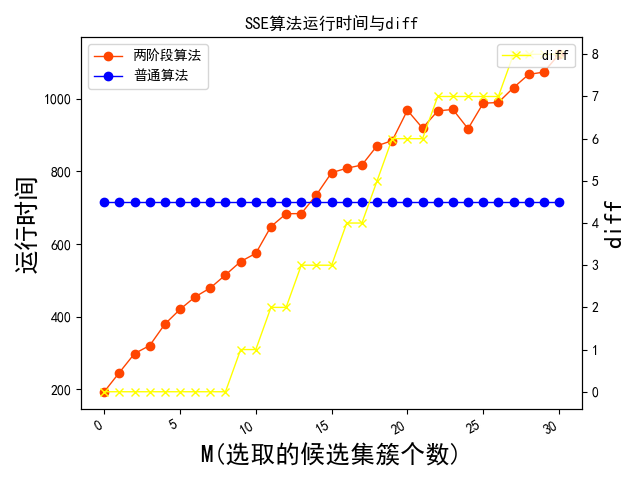
\includegraphics[width=2in]{fig/sse算法运行时间与diff.png}
\label{fig:diff1}
\end{minipage}%
}%
\subfigure[AVX的执行时间和准确率.]{
\begin{minipage}[t]{0.33\linewidth}
\centering
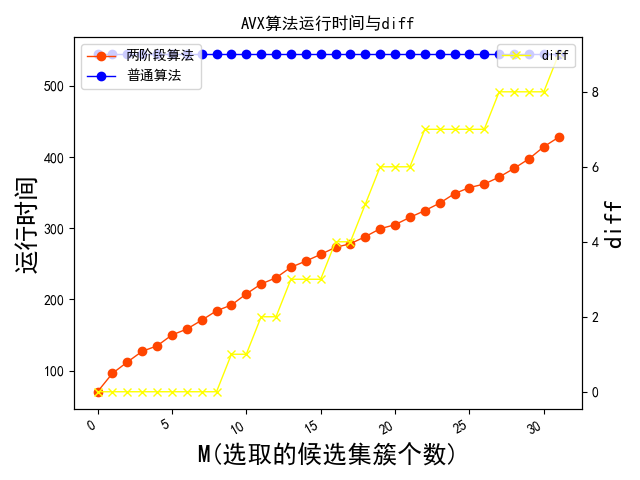
\includegraphics[width=2in]{fig/avx算法运行时间与diff.png}
\end{minipage}%
}%
\subfigure[OpenMP的执行时间和准确率.]{
\begin{minipage}[t]{0.33\linewidth}
\centering
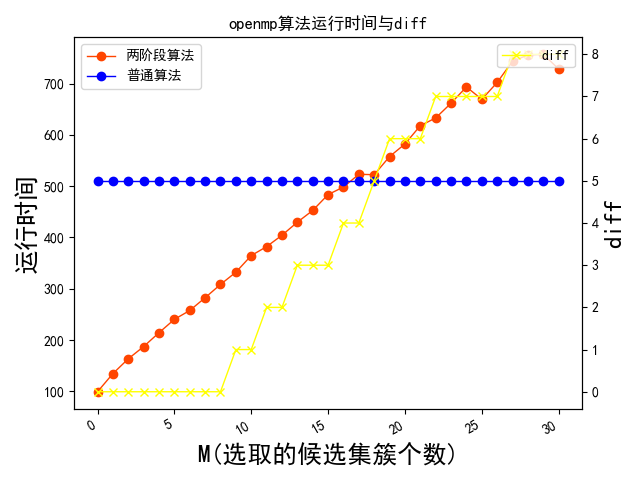
\includegraphics[width=2in]{fig/omp_diff.png}
\end{minipage}%
}%
\centering
\caption{不同并行优化算法的执行时间与准确率对比}
\label{fig:diff}
\end{figure}


表,如表\ref{table:t1}所示。
\begin{table}[!htbp]
  \centering
  \begin{tabular}{ccccccccccc}
  \toprule  
  N/n$\backslash$Algo& naive-conv& naive-pool& omp-conv& omp-pool\\
  \midrule
  64/2& 0.0167& 0.01255& 0.04142& 0.03799\\
  64/4& 0.03599&0.0394& 0.0458& 0.0421\\
  \bottomrule
  \end{tabular}
  \caption{性能测试结果(4线程)(单位:ms)}
  \label{table:t1}
\end{table}

带单元格表格,如表\ref{table:t2}所示。
\begin{table}[!htbp]
  \centering
  \begin{tabular}{|c|c|c|c|c|c|c|}
  \hline
  \multicolumn{2}{|c|}{ \multirow{2}*{$Cost$} }& \multicolumn{5}{c|}{To}\\
  \cline{3-7}
  \multicolumn{2}{|c|}{}&$A$&$B$&$C$&$D$&$E$\\
  \hline
  \multirow{3}*{From}&$B$&7&0&1&3&8\\
  \cline{2-7}
  &$C$&8&1&0&2&7\\
  \cline{2-7}
  &$D$&8&3&2&0&5\\
  \hline
  \end{tabular}
  \caption{结点C距离向量表(无毒性逆转)}
  \label{table:t2}
\end{table}

推荐你们使用这个网站,将数据填进去,设置好格式之后就可以自动生成表格的latex代码。

\href{https://www.tablesgenerator.com/}{TableGenerator}

\section{其他会用到}
\subsection{枚举}
带标号枚举
\begin{enumerate}
  \item 1
  \item 2
\end{enumerate}

不带标号枚举
\begin{itemize}
  \item 1
  \item 2
\end{itemize}

\subsection{公式}

多行公式
\begin{align}
  a+b = a + b \\
  \frac{a+b}{a-b}
\end{align}
\begin{equation}
    a+b = a + b \\
  \frac{a+b}{a-b}
\end{equation}

单行公式:$$\sum^N_{i=1}$$
行内公式:$\sum^N_{i=1}$

推荐你们使用\textit{Mathpix Snip}。是一个公式识别软件,可以自动生成公式对应的latex代码。

\subsection{链接}
参考文献\cite{quinn1994parallel}\cite{golub2014scientific}\cite{joseph2022parallel}
\textbf{超链接}  \href{http://youtube.com/}{YouTube}

\newpage
\bibliographystyle{plain}
\bibliography{reference.bib} 

\end{document}